\documentclass[a4paper]{article}
\usepackage[spanish]{babel}
\title{Taller 1}

\usepackage[utf8]{inputenc}
\usepackage{caratula}
\usepackage{graphicx}
\usepackage{color}
\usepackage{listings}
\usepackage{float}


\setlength{\leftmargin}{2cm}
\setlength{\rightmargin}{2cm}
\setlength{\oddsidemargin}{-1cm}
\setlength{\evensidemargin}{-1cm}
\setlength{\topmargin}{-1cm}
\setlength{\textwidth}{18cm}
\setlength{\textheight}{25cm}

\usepackage{fancyhdr}
\pagestyle{fancy}
\fancyhf{}
\fancyhead[LO,LE]{\scriptsize Trabajo Práctico N$^{\circ}$2}
\fancyhead[RO,RE]{\scriptsize Mancuso, Mataloni, Gonzalez}
\fancyfoot[CE,CO]{\thepage}
\renewcommand{\footrulewidth}{0.4pt}

\usepackage[pdftex, bookmarks=true, colorlinks, citecolor=black, linkcolor=black]{hyperref}
\usepackage{multirow}

\begin{document}

\materia{Teoría de las Comunicaciones}
\submateria{Segundo Cuatrimestre de 2012}
\titulo{Taller de Capa de Red}
\grupo{Taller N$^{\circ}$2}

\integrante{Mancuso, Emiliano}{597/07}{emiliano.mancuso@gmail.com}
\integrante{Mataloni, Alejandro}{706/07}{amataloni@gmail.com}
\integrante{Gonzalez, Matias}{453/07}{curtu\_infinito73@hotmail.com}

\maketitle

\newpage

\addcontentsline{toc}{section}{Índice}

% Main project


\newpage

\section{Primera consigna}

Para estimar el RTT a distintas partes del mundo tomamos IPs de diferentes partes y utilizamos la implementación de \textit{ping} del ejercicio para medir el tiempo de respuesta.  


\begin{table}[H]
\begin{center}
\begin{tabular}{|c|c|c|c|}
\hline
Direccion & IP & Lugar & Distancia(km) \\
\hline
www.portal.gub.ui & 200.40.200.36 & Montevideo, Uruguay & 214 \\
\hline
www.presidencia.gov.co & 190.27.253.9 & Bogota, Colombia & 4627\\
\hline
www.usa.gov & 72.247.242.57 & New York, EEUU & 8671\\
\hline
www.rusopedia.rt.com & 212.24.56.190 & Moscu, Rusia & 13500 \\
\hline
www.jnto.go.gp & 210.165.34.236 & Tokio, Japon  & 18500\\
\hline
\end{tabular}

\end{center}
\end{table}

Para minimizar los posibles errores realizamos varias veces el experimento y en diferentes momentos del día, tomando luego el promedio de los mismos. \\

\begin{figure}[H]
  \centering
  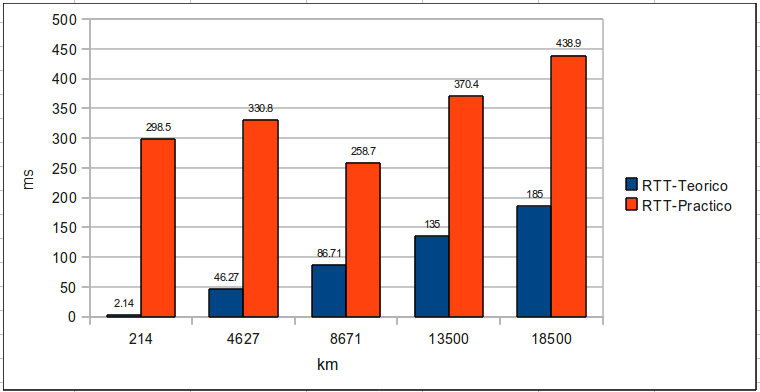
\includegraphics[scale=0.60]{graficos/comparacionRTT.png}
  \caption{Comparacion RTT teorico vs RTT practico }
\end{figure}


Lo que podemos observar en el gráfico es la gran diferencia entre el RTT teórico (calculado suponiendo un enlace punto a punto directo con el IP) y el práctico. Con estos podemos corroborar la existencia de un \textit{delay de red} muy elevado. Esto sucede por varias razones:
\begin{itemize}
	\item No existe enlace punto a punto con cada IP. El paquete enviado debe pasar por varios \textit{routers} antes de llegar al IP elegido.
	\item Cada \textit{router} agrega un delay correspondiente a la sobrecarga o congestión de la red en el momento en el que tiene que \textit{forwardear} el paquete. 
\end{itemize}

En el gráfico podemos notar algo que en un principio nos parecio \textit{raro}. El RTT práctico a EEUU, aunque la distancia es mayor que a Uruguay, es bastante menor. Esto se debe a que no contamos con un enlace directo a Uruguay, sino que el paquete da varios saltos para alcanzar el destino. No así con los EEUU, país con el cual tenemos un enlace más directo.  


\newpage
\section{Segunda}

 Para el desarrollo del taceroute lo que hicimos fue implmentar el algoritmo que se describia en las
 diapositivas del taller.
 Es decir que crear un paquete IP-ICMP y le configurabamos el ttl en 1 y lo enviabamos, luego lo 
 incrementabamos y volviamos a enviar hasta llegar al host deseado.
 
 \subsection{Pruebas}
 Las pruebas para el traceroute se realizaron a los siguientes hosts: yahoo.com, yahoo.com.ar, 
 google.com, google.com.ar y dc.uba.ar.
 
 %~ Primero mostramos las pruebas de cada destino mostrando una ruta general o promedio, es decir cual fue
 %~ la que mas salio.
 
 \begin{table}[!htb]
 	\begin{center}
 	\begin{tabular}{|c|c|c|c|c|}
 	  \hline
 	  ttl & \multicolumn{2}{|c|}{3-5 AM} & \multicolumn{2}{|c|}{7-9 PM} \\\hline
	  1 	&		186.136.215.1 	&	 186.136.215.1 	&	186.137.226.1	&	186.137.226.1	\\ \hline
	  2 	&		186.136.215.1 	&	 \ * &	 \ * 	&	 \ * 	\\ \hline
	  3 	&		186.136.215.1 	&	 \ * &	 \ * 	&	 \ * 	\\ \hline
	  4 	&		186.136.215.1 	&	 \ * &	 \ * 	&	 \ * 	\\ \hline
	  5 	&	 200.89.165.133 	&	 200.89.165.133 &	200.89.165.177	&	200.89.165.157	\\ \hline
	  6 	&	 200.89.165.150 	&	 200.89.165.150	&	200.89.165.150	&	200.89.165.150	\\ \hline
	  7 	&		208.50.25.97 	&	 208.50.25.97	&	208.178.245.21	&	208.50.25.65	\\ \hline
	  8 	&		206.57.3.210 	&	 206.57.3.210	&	67.16.146.149	&	206.57.3.210	\\ \hline
	  9 	&		216.115.100.10 	&	 216.115.100.10 &	67.16.164.26	&	216.115.104.124	\\ \hline
	  10 	&	 216.115.100.7 	&	 216.115.100.7 &	67.16.145.118	&	216.115.100.3	\\ \hline
	  11 	&	 98.138.144.29 	&	 98.138.144.29 &	208.48.239.254	&	98.138.144.29	\\ \hline
	  12 	&		98.138.93.5		&	 98.138.93.5 &	216.115.107.87	&	98.138.93.5	\\ \hline
	  13 	&		98.138.240.32 	&	 98.138.240.32 &	67.195.128.79	&	98.138.240.16	\\ \hline
	  14 	&		98.138.253.109 	&	 98.138.253.109 &	76.13.244.13	&	98.138.253.109	\\ \hline
	  15	&		&		&	72.30.38.140	&		\\ \hline


 	 \end{tabular}   
 	 \vspace{0pt}
 	 \caption{Recorridos a yahoo.com}
 	\end{center}
 	\label{tab:yahoo.com}
 \end{table}
 
 
 
  \begin{table}[!htb]
 	\begin{center}
 	\begin{tabular}{|c|c|c|c|c|}
 	  \hline
 	  ttl & \multicolumn{2}{|c|}{3-5 AM} & \multicolumn{2}{|c|}{7-9 PM}\\ \hline
	  1 & 186.136.215.1 & 186.136.215.1 & 186.137.226.1 & 186.137.226.1\\ \hline
	  2 & 186.136.215.1 &  \ * & \ *  &  \ * \\ \hline
	  3 & 186.136.215.1 &  \ *  &  \ *  &  \ * \\ \hline
	  4 &  \ *  &  \ *  &  \ *  &  \ * \\ \hline
	  5 & 200.89.165.185 & 200.89.165.185 & 200.89.165.189 & 200.89.165.137\\ \hline
	  6 & 200.89.165.150 & 200.89.165.150 & 200.89.165.150 & 200.89.165.150\\ \hline
	  7 & 64.214.130.253 & 64.214.130.253 & 208.50.25.65 & 64.209.94.69\\ \hline
	  8 & 64.215.30.22 & 64.215.30.22 & 64.215.30.22 & 67.16.163.90\\ \hline
	  9 & 216.115.97.199 & 216.115.97.199 & 216.115.97.199 & 67.17.72.14\\ \hline
	  10 & 216.115.100.31 & 216.115.100.31 & 216.115.100.29 & 64.211.206.210\\ \hline
	  11 & 98.139.128.19 & 98.139.128.19 & 98.139.232.99 & 216.115.107.61\\ \hline
	  12 & 98.139.128.63 & 98.139.128.63 & 98.139.128.59 & 209.131.32.19\\ \hline
	  13 & 98.139.129.93 & 98.139.129.93 & 98.139.129.63 & 68.180.206.184\\ \hline
	  14 & 98.139.102.145 & 98.139.102.145 & 98.139.102.145 & \\ \hline

 	 \end{tabular}   
 	 \vspace{0pt}
 	 \caption{Recorridos a yahoo.com.ar}
 	\end{center}
 	\label{tab:yahoo.com.ar}
 \end{table}
 
 \begin{table}[!htb]
 	\begin{center}
 	\begin{tabular}{|c|c|c|c|c|}
 	  \hline
 	  ttl & \multicolumn{2}{|c|}{3-5 AM} & \multicolumn{2}{|c|}{7-9 PM} \\ \hline
	  1 & 186.136.215.1 & 186.136.215.1 & 186.137.226.1 & 186.137.226.1 \\ \hline
	  2 &  \ * &  \ * &  \ * & 186.137.226.1\\ \hline
	  3 &  \ * &  \ * &  \ * &  \ * \\ \hline
	  4 &  \ * &  \ * &  \ * &  \ * \\ \hline
	  5 & 200.89.165.133 & 200.89.165.189 & 200.89.165.177 & 200.89.165.133 \\ \hline
	  6 & 200.89.165.130 & 200.89.165.130 & 200.89.165.130 & 200.89.165.5 \\ \hline
	  7 & 200.89.165.222 & 200.89.165.222 & 200.89.165.222 & 200.89.165.250 \\ \hline
	  8 &  \ *  &  \ *  & 200.49.159.254 & 200.49.159.254 \\ \hline
	  9 & 209.85.251.86 & 209.85.251.86 & 209.85.251.86 & 209.85.251.86 \\ \hline
	  10 & 209.85.251.194 & 209.85.251.194 & 209.85.251.194 & 209.85.251.194 \\ \hline
	  11 & 173.194.42.14 & 173.194.42.0 & 173.194.42.0 & 173.194.42.17 \\ \hline

 	 \end{tabular}   
 	 \vspace{0pt}
 	 \caption{Recorridos a google.com}
 	\end{center}
 	\label{tab:google.com}
 \end{table}
 
\begin{table}[!htb]
 	\begin{center}
 	\begin{tabular}{|c|c|c|c|c|}
 	  \hline
 	  ttl & \multicolumn{2}{|c|}{3-5 AM} & \multicolumn{2}{|c|}{7-9 PM} \\ \hline
	  1 & 186.136.215.1 & 186.136.215.1 &  \ *  &  \ * \\ \hline
	  2 &  \ *  &  \ *  & 186.137.226.1 & 186.137.226.1\\ \hline
	  3 &  \ *  &  \ *  & 186.137.226.1 &  \ * \\ \hline
	  4 &  \ *  &  \ *  &  \ *  &  \ * \\ \hline
	  5 & 200.89.165.185 & 200.89.165.177 & 200.89.165.165 & 200.89.165.177\\ \hline
	  6 & 200.89.165.5 & 200.89.165.130 & 200.89.165.130 & 200.89.165.5\\ \hline
	  7 & 200.89.165.250 & 200.89.165.222 & 200.89.165.222 & 200.89.165.250\\ \hline
	  8 &  \ *  &  \ *  & 200.49.159.254 & 200.49.159.254\\ \hline
	  9 & 209.85.251.86 & 209.85.251.86 & 209.85.251.86 & 209.85.251.86\\ \hline
	  10 & 209.85.251.194 & 209.85.251.194 & 209.85.251.194 & 209.85.251.194\\ \hline
	  11 & 173.194.42.23 & 173.194.42.31 & 173.194.42.31 & 173.194.42.23\\ \hline
 	 \end{tabular}   
 	 \vspace{0pt}
 	 \caption{Recorridos a google.com.ar}
 	\end{center}
 	\label{tab:gootle.com.ar}
 \end{table}

 \begin{table}[!htb]
 	\begin{center}
 	\begin{tabular}{|c|c|}
 	  \hline
 	  ttl &  \\ \hline
	  1	&	 \ * 	\\ \hline
	  2	&	186.136.215.1	\\ \hline
	  3	&	186.136.215.1	\\ \hline
	  4	&	186.136.215.1	\\ \hline
	  5	&	200.89.165.181	\\ \hline
	  6	&	200.89.165.5	\\ \hline
	  7	&	200.89.165.250	\\ \hline
	  8	&	200.49.69.165	\\ \hline
	  9	&	190.220.179.5	\\ \hline
	  10	&	190.220.176.26	\\ \hline
	  11	&	190.220.179.126	\\ \hline
	  12	&	 \ * 	\\ \hline
	  13	&	157.92.47.13	\\ \hline
	  14	&	 \ * 	\\ \hline
	  15	&	 \ * 	\\ \hline
	  16	&	 \ * 	\\ \hline
	  17	&	 \ * 	\\ \hline
	  32	&	 \ * 	\\ \hline
	  64	&	 \ * 	\\ \hline
 	 \end{tabular}   
 	 \vspace{0pt}
 	 \caption{Rutas a dc.uba.ar}
 	\end{center}
 	\label{tab: dc.uba.ar}
 \end{table}
 
  \clearpage
 \subsection{Analisis Pruebas}
 
 Dentro de las pruebas se pueden presenciar momentos en que las rutas no se muestran, en donde aparece un *.
 Esto se debe que se cumplio el timeout de espera de la respuesta al enviar el paquete ICMP, las razones de
 esto pueden ser varias. 
 
 
 En casos como mencionamos anteriormente el host no respondio o no lo hizo en el tiempo esperado.
 Desde un pensamiento basico, sin tener en cuenta argumentos de seguridad, esto se puede deber a que 
 el host este demasiado ocupado como para responder o que se pierda el paquete de respuesta, haciendo que se cumpla el timeout.
 
 En los casos donde los host no alcanzados se encuentran entre los primeros 4 hops esto es cierto,
 porque en otros intentos las ruta se muestran, y son siempre IP similares a las del host que ejecuta el traceroute. La conclusion que obtuvimos es que se trata de las ips del proveedor de internet
 y que responde varias veces porque esta trabajando en la red interna.
  
 En otros casos, como las ultimas rutas del traceroute a \textit{dc.uba.ar} se muestran solo timeouts, para asegurarnos que los mismos no se debian a las razones anteriores seteamos el timeout con valores altos y varios reintentos en el envio de 
de un paquete a un host. Como no obtuvimos diferencias y nunca se pudieron ver las rutas llegamos a la conclusion de que no hay un accesso 'autorizado', es decir que el acceso a ese host esta 
 bloqueado. Posiblemente por un firewall o alguna otra herramienta de proteccion y/o medida  de seguridad. 
 Investigando en internet encontramos  que esto se puede hacer si, por ejemplo en el host se bloquean 
 algunos paquetes hacia los puertos que usa el traceroute, o si el host se configura para no responder
 los  \textit{time exceeded}, que son los tipo de paquetes que utilizamos para implementar el traceroute.
 
 En el caso de las pruebas a \textit{dc.uba.ar} nunca logramos obtener un paquete ICMP del tipo 
 \textit{echo replay}
 es decir que el trace route no termina. En las pruebas con implmentacion tradicionales como el traceroute 
 de linux, el mismo setea un cantidad maxima de hops para terminar la ejecucion del programa. En nuestras 
 pruebas dejamos incluso correr hasta un ttl de mas de 64, que es el ttl que usa por defecto scapy al crear 
 un paqute ICMP, y no obtuvimos respuesta.
 
 
 Por otro lado en los casos en los que se nota que la ruta varia llegamos a la conclusion de que podia ser por una cuestion
 de cantidad de trafico y uso, pues mas de una vez las rutas eran distintas y muchas veces se mostraban 
 rutas ya recorridas.
 Entonces pensamos que al estar un host ocupado el paquete es dirigido hacia otros host. Lo que si notamos es que en nuestras pruebas  a partir de ciertos host el recorrido era el mismo, es
 decir que un cambio en el host X  por el Y la  cadena de host siguientes a Y en general era la misma.
 
 
 \subsubsection{Otros Casos:}
 
 
 Mientras realizabamos al implementacion y luego al hacer las pruebas a uno de los integrantes el 
 traceroute  solo respondia \textit{timeout} de a largos ratos o siempre despues de 1 o 2 hops.
 Comparando con el traceroute de linux, este funcionaba correctamente y nos dabamos cuenta que algo malo estaba
 sucediendo, en un principio pensamos que era la implmentacion lo que nos llevo a probar varias formas reintentar 
 antes de reenviar un paquete, incluso a ver si se podia realizar esos intentos con un intervalo de 
 espera.
 Estas modificaciones presentaron algunas mejoras pero seguia mostrando solo \textit{timeout} o de a largos
 intervalos y ademas la espera entre reintentos debia ser muy amplia (aproximadamente de 5 segundos).
 Luego de varias pruebas se decidio probar la implementacion sin conexion al router es decir directamente
 al modem. El problema se soluciono y al programa funcionaba correctamente.
 Creemos que el router tiene en su configuracion despachar o no responder mensajes \textit{time exceeded} cuando
 los mismo son muchos en un intervalo corto.
 
 
 Servidores con mas de una IP, tambien nos sucedio que una de las primeras implementaciones del traceroute
 comparaba por el nombre de host ingresado y no controlaba el tipo de mensaje respondido, en busqueda
 de un \textit{echo replay}. Por estas razones en host como \textit{google.com} el programa a veces no 
 terminaba pues esperaba hasta encontrar el host ingresado y otras veces tardaba algunos hops mas hasta 
 que contestara el un host en particular, mientras los echo replay los envian otros.

\newpage
\section{Modo de uso}

Para correr los diferentes ejercicios:\\
\begin{itemize}
\item RTT: " ./2\_rtt.py www.google.com 5". Como primer parametro la IP o host y como segundo la cantidad de veces a correr ping para sacar un promedio
\item Traceroute: " ./3\_traceroute.py  www.facebook.com". Como unico parametro la IP o host. 
\end{itemize}

\end{document}
